\documentclass[leqno]{article}
% Shared QBT/Soln pack preamble for resources.danieljsmith.org.
\usepackage{graphicx}
\usepackage{dsfont}
\usepackage{mathtools}
\usepackage{amssymb}
\usepackage{amsmath}
\usepackage{amsthm}
\usepackage{float}
\usepackage{ragged2e}
\usepackage{tensor}
\usepackage{fancyhdr}
\usepackage{empheq}
\usepackage[most]{tcolorbox}
\usepackage{enumitem}
\usepackage{dirtytalk}
\usepackage{marginnote}
\usepackage{microtype}
\usepackage[
  a4paper,
  left=0.8in,
  right=1in,
  top=1in,
  bottom=0.5in,
  headheight=14pt,
  headsep=0.4in
]{geometry}
\setlength{\parindent}{0cm}

% TikZ / PGFPlots
\usepackage{pgfplots}
\pgfplotsset{compat=1.18}
\usepgfplotslibrary{fillbetween, polar}
\usetikzlibrary{calc, positioning}
\usetikzlibrary{angles, quotes}
\usetikzlibrary{arrows.meta}
\usetikzlibrary{decorations.pathreplacing, decorations.markings}
\usetikzlibrary{patterns}
\usetikzlibrary{intersections}

% Links and contents
\usepackage[colorlinks=true,linkcolor=black,citecolor=magenta,urlcolor=black]{hyperref}%
\urlstyle{same}

% Pack macros
\RenewDocumentCommand{\marks}{o m}{%
  \IfValueTF{#1}%
    {\marginnote{\raggedright\textbf{[#2]}}[#1]}%
    {\marginnote{\raggedright\textbf{[#2]}}}%
}

\newcommand{\vspacerule}[2]{%
  \par\vspace*{#1}%
  \noindent\hrulefill\par
  \vspace*{#2}%
}

\definecolor{scarlet}{RGB}{205, 40, 75}

% Worked-solution box, adapted from the TMUA worked-solutions box. A white breakable box with a left scarlet rule and no surrounding
% frame or tint. A part that breaks fills the rest of its page, so the rule
% runs to the bottom margin; the unbroken or last part ends in a short
% horizontal foot rule so a solution visibly stops. Unlike the TMUA box there
% is no answer label and no extra \parskip: these solutions mix \\ line breaks
% with blank lines, so paragraph skips would make the spacing uneven. The box
% does not grow to the left, so the rule sits at the text edge; growing to the
% right keeps the usable line width close to the old tcolorbox Solution box.
\newtcolorbox{djsSolution}{%
  enhanced, breakable, frame hidden, sharp corners, colback=white,
  height fixed for=first and middle, height fill,
  extras unbroken and last={natural height},
  borderline west={2.2pt}{0pt}{scarlet},
  left=11pt, right=0pt, top=5pt, bottom=13pt,
  before skip=13pt, after skip=4pt,
  grow to right by=10mm,
  overlay unbroken and last={%
    \fill[scarlet] (frame.south west)
      rectangle ([xshift=3.5cm, yshift=2.2pt]frame.south west);},
  before upper={{\color{scarlet}\bfseries Solution}\par\vspace{4pt}}}

% Optional smaller figure inside a solution box. \scalebox shrinks node text
% with the drawing. Not applied to existing figures.
\newcommand{\SolnFigureScale}{0.85}
\newsavebox{\djsSolnFigureBox}
\newenvironment{djsSolutionFigure}
  {\par\vspace{4pt}\begin{center}\begin{lrbox}{\djsSolnFigureBox}}
  {\end{lrbox}\scalebox{\SolnFigureScale}{\usebox{\djsSolnFigureBox}}%
   \end{center}\vspace{2pt}\par}

\newcommand{\cxl}[2]{%
  \tikz[baseline=(X.base)]{%
    \node[inner sep=0pt, outer sep=0pt, text=#1] (X) {$#2$};
    \draw[#1, line width=0.4pt] (X.south west)--(X.north east);
  }%
}

% Page-style hook run at the contents page and each question's opening page.
% A no-op for QBT packs; \djsSolnHeader points it at the fancy header.
\newcommand{\djsQuestionPageStyle}{}

\newcommand{\questionitem}{%
  \djsQuestionPageStyle
  \item\phantomsection
  \addcontentsline{toc}{section}{Question \number\value{enumi}}%
}

\renewcommand{\contentsname}{Questions}

\newcommand{\djsPackHeader}[1]{%
  \pagestyle{fancy}%
  \fancyhead{}%
  \fancyfoot{}%
  \renewcommand{\headrulewidth}{0.9pt}%
  \lhead{#1}%
  \chead{}%
  \rhead{\href{https://danieljsmith.org}{danieljsmith.org}}%
}

\newcommand{\djsQbtHeader}[1]{%
  \djsPackHeader{#1}%
}

% Solutions packs show the header only on the contents page and each
% question's opening page, so it never appears part-way through a solution.
% \thispagestyle marks the next page shipped out, which is the question's
% page because every solution question starts after a \newpage.
\newcommand{\djsSolnHeader}[1]{%
  \djsPackHeader{\textit{Solutions} - #1}%
  \pagestyle{empty}%
  \renewcommand{\djsQuestionPageStyle}{\thispagestyle{fancy}}%
}

\newcommand{\djsFrontMatter}{%
  \djsQuestionPageStyle
  \vspace*{20pt}%
  \tableofcontents
  \newpage
}


\djsSolnHeader{Elastic Potential Energy}

\begin{document}
\djsFrontMatter
\begin{enumerate}[
  label=\textbf{\arabic*.},
  leftmargin=*,
  topsep=0pt,
  partopsep=0pt,
  parsep=0pt
]

% ---- Question 1 ----
\questionitem
% [Source: _QBT___Solns__Elastic_Potential_Energy, Q1]

One end of a light elastic string, of natural length $2a$ and modulus of elasticity $2mg$, is attached to a fixed point $O$. The other end of the string is attached to a particle $P$ of mass $m$. The string is vertical with $P$ directly above $O$. The particle $P$ is pulled vertically upwards until the extension of the string is $2a$. The particle $P$ is then released from rest. \\
\begin{enumerate}[label=\textbf{(\alph*)}]
  \item Find the speed of $P$ when it is at a distance $\dfrac{3}{2}a$ above $O$. \marks{3} \\
  \item Find the initial acceleration of $P$ when it is released from rest. \marks{2} \\
\end{enumerate}

\vspace*{10pt}

\begin{tcolorbox}[colback=white, colframe=scarlet, title={\textbf{Solution}}, breakable, grow to left by=6mm, grow to right by=10mm]
\begin{enumerate}[label=\textbf{(\alph*)}, start=1]
  \item The natural length of the string is $2a$.

Initially the extension is $2a$, so the initial length is
\[
2a+2a=4a
\]
Hence initially $P$ is $4a$ above $O$.

When $P$ is $\dfrac{3}{2}a$ above $O$, the length of the string is $\dfrac{3}{2}a<2a$, so the string is slack. Therefore at this point the elastic potential energy is $0$.

Use conservation of mechanical energy:
\[
KE_0+GPE_0+EPE_0=KE_1+GPE_1+EPE_1
\]
Initially, $P$ is released from rest, so $KE_0=0$.

Initial elastic potential energy:
\[
EPE_0=\frac{\lambda x^2}{2l}
=\frac{(2mg)(2a)^2}{2(2a)}
=2mga
\]
where $\lambda=2mg$, $x=2a$, and $l=2a$.

Taking gravitational potential energy relative to $O$,
\[
GPE_0=mg(4a),\qquad GPE_1=mg\left(\frac{3a}{2}\right)
\]
Also,
\[
KE_1=\frac12 mv^2,\qquad EPE_1=0
\]
So
\begin{align*}
0+4mga+2mga&=\frac12 mv^2+\frac32 mga+0 \\
6mga&=\frac12 mv^2+\frac32 mga \\
\frac12 mv^2&=\frac92 mga
\end{align*}
Hence
\[
v^2=9ag
\]
so
\[
v=3\sqrt{ag}
\]
Therefore the speed of $P$ is $3\sqrt{ag}$.

  \item Initially, the extension is $2a$, so the tension is
\[
T=\frac{\lambda x}{l}
=\frac{(2mg)(2a)}{2a}
=2mg
\]
This tension acts downward, towards $O$. The weight $mg$ also acts downward.

So the resultant force on $P$ initially is
\[
2mg+mg=3mg
\]
downward.

Using $F=ma$,
\[
ma=3mg
\]
so
\[
a=3g
\]
Therefore the initial acceleration is $3g$ downward.
\end{enumerate}
\end{tcolorbox}


\newpage

% ---- Question 2 ----
\questionitem
% [Source: _QBT___Solns__Elastic_Potential_Energy, Q2]

A light elastic string has natural length $2.5$ metres and modulus of elasticity $15$ newtons. \\

One end of the elastic string is attached to a particle of mass $0.75\,\mathrm{kg}$. \\

The other end of the elastic string is attached to a fixed point $O$. \\

The particle is released from rest at a point $A$, which is $2.9$ metres vertically below $O$. \\

\begin{enumerate}[label=\textbf{(\alph*)}]
  \item Calculate the elastic potential energy stored in the string when the particle is at $A$. \marks{2} \\
  \item The point $B$ is $4.0$ metres vertically below $O$. \\
  Calculate the gravitational potential energy lost by the particle as it moves from $A$ to $B$. \marks{2} \\
  \item Find the speed of the particle at $B$. \marks{3} \\
  \item The point $C$ is $3.3$ metres vertically below $O$. \\
  Explain, showing any calculations that you make, why the speed of the particle is increasing the first time that the particle is at $C$. \marks{3} \\
\end{enumerate}

\vspace*{10pt}

\begin{tcolorbox}[colback=white, colframe=scarlet, title={\textbf{Solution}}, breakable, grow to left by=6mm, grow to right by=10mm]
\begin{enumerate}[label=\textbf{(\alph*)}, start=1]
  \item The extension of the string at \(A\) is
\[
 x_A=2.9-2.5=0.4\,\mathrm{m}
\]
For an elastic string,
\[
EPE=\frac{\lambda x^2}{2l}
\]
So
\[
EPE_A=\frac{15(0.4)^2}{2(2.5)}=0.48\,\mathrm{J}
\]
Hence the elastic potential energy stored when the particle is at \(A\) is \(0.48\,\mathrm{J}\).

  \item The particle falls from \(2.9\,\mathrm{m}\) below \(O\) to \(4.0\,\mathrm{m}\) below \(O\), so the vertical distance moved down is
\[
4.0-2.9=1.1\,\mathrm{m}
\]
Therefore the gravitational potential energy lost is
\[
mg\times 1.1=0.75\times 9.8\times 1.1=8.085\,\mathrm{J}
\]
Hence the gravitational potential energy lost is \(8.085\,\mathrm{J}\).

  \item At \(B\), the extension is
\[
 x_B=4.0-2.5=1.5\,\mathrm{m}
\]
So the elastic potential energy at \(B\) is
\[
EPE_B=\frac{15(1.5)^2}{2(2.5)}=6.75\,\mathrm{J}
\]
Using the work-energy principle,
\[
KE_A+GPE_A+EPE_A=KE_B+GPE_B+EPE_B
\]
The particle is released from rest, so \(KE_A=0\). Also, from part (b), the loss in GPE from \(A\) to \(B\) is \(8.085\,\mathrm{J}\). Therefore
\[
KE_B=EPE_A+\text{GPE lost}-EPE_B
\]
\[
KE_B=0.48+8.085-6.75=1.815\,\mathrm{J}
\]
Now
\[
\frac12 \times 0.75\times v^2=1.815
\]
so
\[
v^2=\frac{2\times1.815}{0.75}=4.84
\]
\[
v=2.2\,\mathrm{m\,s^{-1}}
\]
Hence the speed of the particle at \(B\) is \(2.2\,\mathrm{m\,s^{-1}}\).

  \item At \(C\), the extension is
\[
 x_C=3.3-2.5=0.8\,\mathrm{m}
\]
So the tension in the string is
\[
T=\frac{\lambda x}{l}=\frac{15\times 0.8}{2.5}=4.8\,\mathrm{N}
\]
This acts upwards.

The weight of the particle is
\[
0.75\times 9.8=7.35\,\mathrm{N}
\]
This acts downwards.

Hence the resultant force is
\[
7.35-4.8=2.55\,\mathrm{N}
\]
downwards, so the acceleration is downwards.

The first time the particle is at \(C\), it is moving downwards because it has fallen from \(A\) towards \(B\). Since the acceleration is also downwards, the acceleration is in the same direction as the motion.

Therefore the speed is increasing the first time that the particle is at \(C\).
\end{enumerate}
\end{tcolorbox}


\newpage

% ---- Question 3 ----
\questionitem
% [Source: _QBT___Solns__Elastic_Potential_Energy, Q3]

A particle $P$ of mass $m$ is attached to one end of a light elastic string of natural length $a$ and modulus $2mg$. The other end of the string is attached to a fixed point $O$ on a rough plane inclined at $30^\circ$ to the horizontal. \\

The string lies along a line of greatest slope, with $O$ below $P$. The particle is initially at rest on the plane with the string at its natural length. \\

The coefficient of friction between $P$ and the plane is $\dfrac{1}{\sqrt{3}}$. \\

The particle is projected up the plane, away from $O$, with speed $\sqrt{\dfrac{3ga}{2}}$. \\

Find the greatest extension of the string during the subsequent motion. \marks{5} \\

\vspace*{10pt}

\begin{tcolorbox}[colback=white, colframe=scarlet, title={\textbf{Solution}}, breakable, grow to left by=6mm, grow to right by=10mm]
Let \(x\) be the greatest extension of the string.

While the particle moves up the plane to this point, it is moving upwards, so friction acts down the plane. Since the string lies along the plane, it has no component perpendicular to the plane, so
\[
R=mg\cos 30^\circ=\frac{\sqrt{3}}{2}mg
\]
Hence the friction force is
\[
\mu R=\frac{1}{\sqrt{3}}\times \frac{\sqrt{3}}{2}mg=\frac{1}{2}mg
\]

Take the initial position as the zero level for gravitational potential energy, and take work done by friction as negative.

Using the work-energy principle,
\[
KE_0+GPE_0+EPE_0+W_{\text{fric}}=KE_1+GPE_1+EPE_1
\]
we have
\[
KE_0=\frac12 m\left(\sqrt{\frac{3ga}{2}}\right)^2=\frac{3mga}{4},
\qquad
KE_1=0
\]
Also, after moving a distance \(x\) up the plane, the vertical rise is \(x\sin 30^\circ=\frac{x}{2}\), so
\[
GPE_0=0,
\qquad
GPE_1=mg\left(\frac{x}{2}\right)=\frac12 mgx
\]
The string starts at natural length, so
\[
EPE_0=0,
\qquad
EPE_1=\frac{\lambda x^2}{2a}
=\frac{(2mg)x^2}{2a}
=\frac{mgx^2}{a}
\]
And the work done by friction is
\[
W_{\text{fric}}=-\left(\frac12 mg\right)x=-\frac12 mgx
\]

Substituting into the energy equation:
\[
\frac{3mga}{4}-\frac12 mgx=\frac12 mgx+\frac{mgx^2}{a}
\]
So
\[
\frac{3mga}{4}=mgx+\frac{mgx^2}{a}
\]
Divide through by \(mg\):
\[
\frac{3a}{4}=x+\frac{x^2}{a}
\]
Multiply through by \(a\):
\[
\frac{3a^2}{4}=ax+x^2
\]
Hence
\[
x^2+ax-\frac{3a^2}{4}=0
\]
Solving this quadratic,
\[
x=\frac{-a\pm\sqrt{a^2+3a^2}}{2}=\frac{-a\pm2a}{2}
\]
So
\[
x=\frac a2 \quad \text{or} \quad x=-\frac{3a}{2}
\]
Since \(x\) is an extension, it must be positive. Therefore
\[
x=\frac a2
\]
Hence the greatest extension of the string is \(\dfrac{a}{2}\).
\end{tcolorbox}


\newpage

% ---- Question 4 ----
\questionitem
% [Source: _QBT___Solns__Elastic_Potential_Energy, Q4]

The points $A$ and $B$ are at the same horizontal level and are $24a$ apart. The ends of a light elastic string, of natural length $18a$ and modulus of elasticity $\lambda$, are attached to $A$ and $B$. A particle $P$ of mass $m$ is attached to the midpoint of the string. The system is in equilibrium with $P$ at a distance $5a$ below $M$, the midpoint of $AB$. \\
\begin{enumerate}[label=\textbf{(\alph*)}]
  \item Find $\lambda$ in terms of $m$ and $g$. \marks{3} \\
\end{enumerate}
The particle $P$ is pulled down vertically and released from rest from a position $9a$ below $M$. \\
\begin{enumerate}[label=\textbf{(\alph*)}, resume]
  \item Find, in terms of $a$ and $g$, the speed of $P$ as it passes through its equilibrium position. \marks{4} \\
\end{enumerate}

\vspace*{10pt}

\begin{tcolorbox}[colback=white, colframe=scarlet, title={\textbf{Solution}}, breakable, grow to left by=6mm, grow to right by=10mm]
\begin{enumerate}[label=\textbf{(\alph*)}, start=1]
  \item At equilibrium,
\[
AM=12a,\qquad MP=5a
\]
so
\[
AP=\sqrt{(12a)^2+(5a)^2}=13a
\]
Hence the actual length of the whole string is
\[
2\times 13a=26a
\]
so its extension is
\[
26a-18a=8a
\]
Let the tension in each side be $T$. Using $T=\dfrac{\lambda x}{l}$ for a string of natural length $l$ and extension $x$,
\[
T=\frac{\lambda(8a)}{18a}=\frac{4\lambda}{9}
\]
If $\theta$ is the angle each side makes with the horizontal, then from the $5$-$12$-$13$ triangle,
\[
\sin\theta=\frac{5}{13}
\]
Resolving vertically for equilibrium,
\begin{align*}
2T\sin\theta&=mg\\
2\left(\frac{4\lambda}{9}\right)\left(\frac{5}{13}\right)&=mg\\
\frac{40\lambda}{117}&=mg
\end{align*}
Therefore
\[
\lambda=\frac{117mg}{40}
\]
So $\lambda=\dfrac{117mg}{40}$.

  \item When $P$ is $9a$ below $M$,
\[
AP=\sqrt{(12a)^2+(9a)^2}=15a
\]
So the whole string has length
\[
2\times 15a=30a
\]
and therefore its extension is
\[
30a-18a=12a
\]
For a light elastic string,
\[
EPE=\frac{\lambda x^2}{2l}
\]
where $l$ is the natural length and $x$ is the extension.

Initially,
\begin{align*}
EPE_0&=\frac{\lambda(12a)^2}{2(18a)}\\
&=4\lambda a
\end{align*}
At the equilibrium position, the extension is $8a$, so
\begin{align*}
EPE_1&=\frac{\lambda(8a)^2}{2(18a)}\\
&=\frac{16\lambda a}{9}
\end{align*}
Hence the decrease in elastic potential energy is
\[
4\lambda a-\frac{16\lambda a}{9}=\frac{20\lambda a}{9}
\]
From the release point to equilibrium, $P$ rises by
\[
9a-5a=4a
\]
so its gravitational potential energy increases by
\[
4mga
\]
Using
\[
KE_0+GPE_0+EPE_0=KE_1+GPE_1+EPE_1
\]
and noting that it is released from rest, we get
\begin{align*}
\frac{20\lambda a}{9}&=4mga+\frac12 mv^2
\end{align*}
Substitute $\lambda=\dfrac{117mg}{40}$:
\begin{align*}
\frac{20a}{9}\cdot \frac{117mg}{40}&=4mga+\frac12 mv^2\\
\frac{13}{2}mga&=4mga+\frac12 mv^2\\
\frac{5}{2}mga&=\frac12 mv^2\\
v^2&=5ag
\end{align*}
Therefore
\[
v=\sqrt{5ag}
\]
So the speed of $P$ as it passes through equilibrium is $\sqrt{5ag}$.
\end{enumerate}
\end{tcolorbox}


\newpage

% ---- Question 5 ----
\questionitem
% [Source: _QBT___Solns__Elastic_Potential_Energy, Q5]

A light elastic string has natural length $3a$ and modulus of elasticity $9mg$. \\
One end of the string is attached to a fixed point $O$. A particle $P$ of mass $m$ is attached to the other end. \\
The particle hangs freely in equilibrium at the point $E$, vertically below $O$. \\
\begin{enumerate}[label=\textbf{(\alph*)}]
  \item Find the length $OE$. \marks{4} \\
\end{enumerate}
The particle is then pulled vertically downwards from $E$ to a point $A$, where $OA = \dfrac{16a}{3}$, and released from rest. \\
The resistance to the motion of $P$ is a constant force of magnitude $\dfrac{1}{4}mg$. \\
\begin{enumerate}[label=\textbf{(\alph*)}, resume]
  \item Find, in terms of $a$ and $g$, the speed of $P$ as it passes through $E$. \marks{7} \\
\end{enumerate}
The particle is now held at $O$ and released from rest. \\
The resistance to the motion of $P$ is again a constant force of magnitude $\dfrac{1}{4}mg$. \\
The speed of $P$ is greatest when it is at the point $B$. \\
\begin{enumerate}[label=\textbf{(\alph*)}, resume]
  \item Find the distance $OB$. \marks{4} \\
\end{enumerate}

\vspace*{10pt}

\begin{tcolorbox}[colback=white, colframe=scarlet, title={\textbf{Solution}}, breakable, grow to left by=6mm, grow to right by=10mm]
\begin{enumerate}[label=\textbf{(\alph*)}, start=1]
  \item Let the extension of the string in equilibrium be \(e\).

The tension is
\[
T=\frac{\lambda e}{3a}
=\frac{9mg\,e}{3a}
=\frac{3mge}{a}
\]

At equilibrium, the tension balances the weight, so
\[
\frac{3mge}{a}=mg
\]
\[
e=\frac{a}{3}
\]

Hence the length of the string is
\[
OE=3a+\frac{a}{3}=\frac{10a}{3}
\]

So \(OE=\dfrac{10a}{3}\).

  \item From part (a), the extension at \(E\) is
\[
OE-3a=\frac{10a}{3}-3a=\frac{a}{3}
\]

At \(A\),
\[
OA=\frac{16a}{3}
\]
so the extension at \(A\) is
\[
\frac{16a}{3}-3a=\frac{7a}{3}
\]

Also,
\[
AE=\frac{16a}{3}-\frac{10a}{3}=2a
\]

For an elastic string, the elastic potential energy is
\[
EPE=\frac{\lambda x^2}{2l}
\]
where \(x\) is the extension and \(l=3a\).

So at \(A\),
\[
EPE_A=\frac{9mg}{2(3a)}\left(\frac{7a}{3}\right)^2=\frac{49}{6}mga
\]
and at \(E\),
\[
EPE_E=\frac{9mg}{2(3a)}\left(\frac{a}{3}\right)^2=\frac{1}{6}mga
\]

Take gravitational potential energy to be zero at \(A\). Then
\[
GPE_A=0,
\qquad
GPE_E=mg(2a)=2mga
\]

The resistance has magnitude \(\dfrac14 mg\) and acts opposite to the motion, so the work done by the resistance from \(A\) to \(E\) is
\[
W_{\text{resistance}}=-\frac14 mg(2a)=-\frac12 mga
\]

Using the work-energy principle,
\[
KE_A+GPE_A+EPE_A+W_{\text{resistance}}=KE_E+GPE_E+EPE_E
\]

Since the particle is released from rest at \(A\),
\[
0+0+\frac{49}{6}mga-\frac12 mga=\frac12 mv^2+2mga+\frac16 mga
\]

So
\[
\frac{46}{6}mga=\frac12 mv^2+\frac{13}{6}mga
\]
\[
\frac12 mv^2=\frac{33}{6}mga=\frac{11}{2}mga
\]
\[
v^2=11ag
\]

Hence the speed as \(P\) passes through \(E\) is
\[
v=\sqrt{11ag}
\]

  \item The particle is released from rest at \(O\).

While the string is slack, there is no tension. The forces are weight \(mg\) downwards and resistance \(\dfrac14 mg\) upwards, so the resultant force is
\[
mg-\frac14 mg=\frac34 mg
\]
downwards.

So at first the particle accelerates downwards and its speed increases.

Once the string becomes taut, let the extension be \(x\). Then the tension is
\[
T=\frac{\lambda x}{3a}=\frac{9mg\,x}{3a}=\frac{3mgx}{a}
\]

The downward resultant force is now
\[
mg-\frac14 mg-T=\frac34 mg-\frac{3mgx}{a}
\]

The speed is greatest when the acceleration is zero, so the resultant force is zero:
\[
\frac34 mg-\frac{3mgx}{a}=0
\]
\[
\frac34=\frac{3x}{a}
\]
\[
x=\frac{a}{4}
\]

For \(x<\dfrac{a}{4}\), the resultant is downward, so the speed is increasing. For \(x>\dfrac{a}{4}\), the resultant is upward, so the speed is decreasing. Therefore the maximum speed occurs when the extension is \(\dfrac{a}{4}\).

Hence
\[
OB=3a+\frac{a}{4}=\frac{13a}{4}
\]

So \(OB=\dfrac{13a}{4}\).
\end{enumerate}
\end{tcolorbox}


\newpage

% ---- Question 6 ----
\questionitem
% [Source: _QBT___Solns__Elastic_Potential_Energy, Q6]

\begin{figure}[H]
    \centering
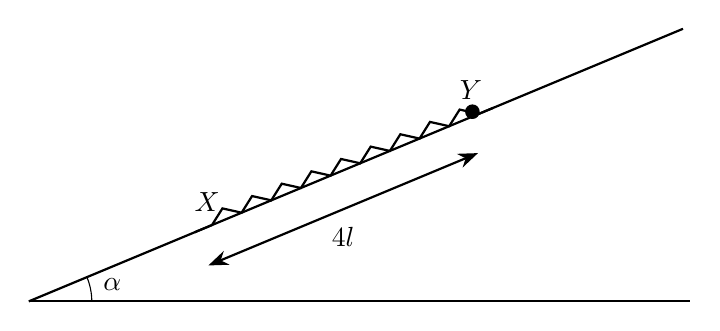
\begin{tikzpicture}[scale=1.2]
\pgfmathsetmacro{\ang}{atan(5/12)}
\def\planeLen{7.5}
\def\xstart{1.9}
\def\lead{0.20}
\def\seg{0.17}
\pgfmathsetmacro{\springLen}{\lead + 17*\seg}
\def\amp{0.12}
\def\measureOff{0.38}

\coordinate (A) at (0,0);
\coordinate (H) at (7.0,0);
\coordinate (Top) at (\ang:\planeLen);
\coordinate (X) at ($(A)+(\ang:\xstart)$);
\coordinate (Y) at ($(X)+(\ang:\springLen)$);
\coordinate (Xm) at ($(X)+(\ang-90:\measureOff)$);
\coordinate (Ym) at ($(Y)+(\ang-90:\measureOff)$);

\draw[thick] (A) -- (H);
\draw[thick] (A) -- (Top);

\begin{scope}[shift={(X)}, rotate=\ang]
  \draw[thick]
    (0,0) -- (\lead,0)
    \foreach \k in {1,...,9} {
      -- ++(\seg,\amp)
      -- ++(\seg,-\amp)
    }
    -- ++(\seg,0);
\end{scope}

\fill[black] ([yshift=2.5pt, xshift=2.5pt]Y) circle (2.2pt);

\draw[{Stealth[length=2.5mm]}-{Stealth[length=2.5mm]}, thick] (Xm) -- (Ym)
  node[midway, below=5pt, fill=white, inner sep=1pt] {$4l$};

\pic["$\alpha$", draw, angle radius=8mm, angle eccentricity=1.35]
  {angle=H--A--Top};

\node[above right, yshift=4pt, xshift=-3.5pt] at (X) {$X$};
\node[above, yshift=4pt, xshift=2.5pt] at (Y) {$Y$};
\end{tikzpicture}
\end{figure}


A light elastic spring has natural length $2l$ and modulus of elasticity $mg$. One end of the spring is attached to a fixed point $X$ on a rough inclined plane. The other end is attached to a package $P$ of mass $m$. \\

The plane is inclined to the horizontal at an angle $\alpha$ where
\[
\tan \alpha = \dfrac{5}{12}
\] 
The package is initially held at the point $Y$ on the plane, where $XY = 4l$. The point $Y$ is higher than $X$ and $XY$ is a line of greatest slope of the plane, as shown. The package is released from rest at $Y$ and moves down the plane. \\

The coefficient of friction between $P$ and the plane is $\dfrac{1}{4}$. \\

By modelling $P$ as a particle, \\
\begin{enumerate}[label=\textbf{(\alph*)}]
  \item show that the acceleration of $P$ at the instant when it is released is
  \[
  \dfrac{15}{13}g
  \]
  down the plane. \marks{5} \\
  \item find, in terms of $g$ and $l$, the speed of $P$ at the instant when the spring first regains its natural length. \marks{6} 
\end{enumerate}

\vspace*{10pt}

\begin{tcolorbox}[colback=white, colframe=scarlet, title={\textbf{Solution}}, breakable, grow to left by=6mm, grow to right by=10mm]
\begin{enumerate}[label=\textbf{(\alph*)}, start=1]
  \item Since
  \[
  \tan\alpha=\frac{5}{12}
  \]
  we have
  \[
  \sin\alpha=\frac{5}{13},\qquad \cos\alpha=\frac{12}{13}
  \]

  Initially the spring has length $4l$ and natural length $2l$, so its extension is
  \[
  4l-2l=2l
  \]
  The modulus of elasticity is $mg$, so the tension is
  \[
  T=\frac{\lambda x}{\text{natural length}}=\frac{mg(2l)}{2l}=mg
  \]
  This tension acts down the plane, towards $X$.

  Since the spring lies along the plane, it has no component perpendicular to the plane. Hence the normal reaction is
  \[
  R=mg\cos\alpha=mg\times\frac{12}{13}=\frac{12mg}{13}
  \]
  So the friction is
  \[
  F=\mu R=\frac14\times\frac{12mg}{13}=\frac{3mg}{13}
  \]
  and this acts up the plane.

  The component of the weight down the plane is
  \[
  mg\sin\alpha=mg\times\frac{5}{13}=\frac{5mg}{13}
  \]

  Therefore the resultant force down the plane is
  \begin{align*}
  T+mg\sin\alpha-F
  &=mg+\frac{5mg}{13}-\frac{3mg}{13}\\
  &=mg+\frac{2mg}{13}\\
  &=\frac{15mg}{13}
  \end{align*}

  Using $F=ma$,
  \[
  ma=\frac{15mg}{13}
  \]
  so
  \[
  a=\frac{15}{13}g
  \]

  Therefore the acceleration is $\dfrac{15}{13}g$ down the plane.

  \item Let the instant of release be state $0$, and let state $1$ be the instant when the spring first regains its natural length.

  The spring length changes from $4l$ to $2l$, so the package moves
  \[
  4l-2l=2l
  \]
  down the plane.

  We use
  \[
  KE_0+GPE_0+EPE_0+\sum W_{\text{other}}=KE_1+GPE_1+EPE_1
  \]
  taking work done against friction as negative.

  Initially the package is at rest, so
  \[
  KE_0=0
  \]
  At the instant when the spring regains its natural length,
  \[
  EPE_1=0
  \]

  The initial extension of the spring is $2l$, so
  \[
  EPE_0=\frac{\lambda x^2}{2\times 2l}=\frac{mg(2l)^2}{4l}=mgl
  \]

  The vertical drop of the package is
  \[
  2l\sin\alpha=2l\times\frac{5}{13}=\frac{10l}{13}
  \]
  so, taking $GPE_1=0$,
  \[
  GPE_0=mg\times\frac{10l}{13}=\frac{10mgl}{13}
  \]

  The friction is constant, with magnitude
  \[
  \frac{3mg}{13}
  \]
  Hence the work done against friction over distance $2l$ is
  \[
  \sum W_{\text{other}}=-\frac{3mg}{13}\times 2l=-\frac{6mgl}{13}
  \]

  Substitute into the energy equation:
  \begin{align*}
  0+\frac{10mgl}{13}+mgl-\frac{6mgl}{13}
  &=\frac12 mv^2+0+0\\
  mgl+\frac{4mgl}{13}
  &=\frac12 mv^2\\
  \frac{17mgl}{13}
  &=\frac12 mv^2
  \end{align*}

  Therefore
  \[
  v^2=\frac{34gl}{13}
  \]
  and so
  \[
  v=\sqrt{\frac{34gl}{13}}
  \]

  Hence the speed is $\sqrt{\dfrac{34gl}{13}}$.
\end{enumerate}
\end{tcolorbox}


\newpage

% ---- Question 7 ----
\questionitem
% [Source: _QBT___Solns__Elastic_Potential_Energy, Q7]

\begin{figure}[H]
    \centering
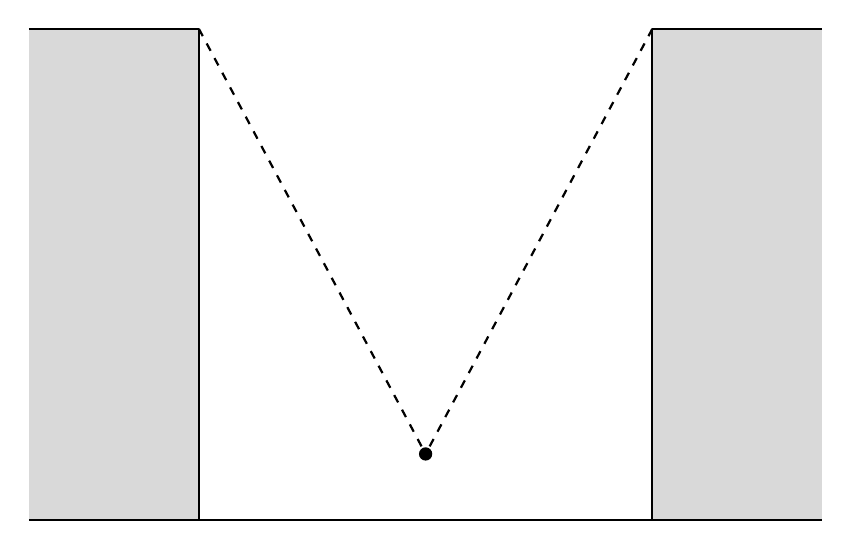
\begin{tikzpicture}[scale=0.12]
\def\depth{52}
\def\halfwidth{24}
\def\outer{42}
\def\starth{7}

\coordinate (Ltop) at (-\halfwidth,\depth);
\coordinate (Rtop) at (\halfwidth,\depth);
\coordinate (Lbase) at (-\halfwidth,0);
\coordinate (Rbase) at (\halfwidth,0);
\coordinate (H) at (0,\starth);

\fill[gray!30] (-\outer,0) rectangle (-\halfwidth,\depth);
\fill[gray!30] (\halfwidth,0) rectangle (\outer,\depth);

\draw[thick] (-\outer,\depth) -- (-\halfwidth,\depth);
\draw[thick] (\halfwidth,\depth) -- (\outer,\depth);
\draw[thick] (-\outer,0) -- (-\halfwidth,0);
\draw[thick] (\halfwidth,0) -- (\outer,0);
\draw[thick] (Ltop) -- (Lbase);
\draw[thick] (Rtop) -- (Rbase);
\draw[thick] (Lbase) -- (Rbase);

\draw[dashed, thick] (Ltop) -- (H);
\draw[dashed, thick] (Rtop) -- (H);
\fill[black] (H) circle (20pt);
\end{tikzpicture}
\end{figure}


A stunt performer is attached to two identical light elastic cords. One end of each cord is fixed to opposite sides of the rim of a vertical shaft, as shown in the diagram above. \\

The performer has mass $80\,\mathrm{kg}$ and is modelled as a particle. Initially the performer is held at rest at the centre of the shaft, $7$ metres above the floor. The shaft is $52$ metres deep and $48$ metres wide. Each elastic cord has natural length $30$ metres and modulus of elasticity $3150\,\mathrm{N}$. \\

The performer is released from rest. \\

\begin{enumerate}[label=\textbf{(\alph*)}]
  \item Show that the speed of the performer when the cords first become slack is $25\,\mathrm{m\,s^{-1}}$ correct to two significant figures. \marks{6} \\
  \item Determine whether the performer is moving up or down when the cords become taut again. \marks{5} \\
\end{enumerate}

\vspace*{10pt}

\begin{tcolorbox}[colback=white, colframe=scarlet, title={\textbf{Solution}}, breakable, grow to left by=6mm, grow to right by=10mm]
\begin{enumerate}[label=\textbf{(\alph*)}, start=1]
  \item The performer is initially at the centre of the shaft, so the horizontal distance to each fixing point is
\[
\frac{48}{2}=24\,\mathrm{m}
\]
and the vertical distance below the rim is
\[
52-7=45\,\mathrm{m}
\]
Hence the initial length of each cord is
\[
\sqrt{24^2+45^2}=\sqrt{2601}=51\,\mathrm{m}
\]
So the initial extension of each cord is
\[
51-30=21\,\mathrm{m}
\]

When the cords first become slack, each cord has its natural length, $30\,\mathrm{m}$.
If the performer is then $h\,\mathrm{m}$ above the floor, the vertical distance below the rim is $52-h$, so
\[
24^2+(52-h)^2=30^2
\]
\[
(52-h)^2=324
\]
Since the performer is still below the rim at this instant,
\[
52-h=18
\]
so
\[
h=34
\]
Therefore the performer has risen
\[
34-7=27\,\mathrm{m}
\]

Using
\[
KE_0+GPE_0+EPE_0=KE_1+GPE_1+EPE_1
\]
and taking the floor as the zero level for GPE,

\begin{align*}
0+80(9.8)(7)+2\left(\frac{3150\times 21^2}{2\times 30}\right)
&=\frac12(80)v^2+80(9.8)(34)+0 \\
5488+46305&=40v^2+26656 \\
25137&=40v^2 \\
v^2&=628.425
\end{align*}

So
\[
v=\sqrt{628.425}=25.1\ldots
\]

Hence the speed when the cords first become slack is $25\,\mathrm{m\,s^{-1}}$ correct to $2$ significant figures.

  \item From part (a), when the cords first become slack the performer is $34\,\mathrm{m}$ above the floor and has
\[
v^2=628.425
\]

While the cords are slack, there is no elastic potential energy, so mechanical energy is exchanged only between KE and GPE.
At the highest point the speed is $0$, so

\begin{align*}
\frac12(80)v^2+80(9.8)(34)&=0+80(9.8)H \\
40v^2+26656&=784H
\end{align*}

Using $v^2=628.425$,
\[
H=34+\frac{628.425}{19.6}\approx 66.1
\]

So the greatest height reached is $66.1\,\mathrm{m}$ above the floor, which is
\[
66.1-52=14.1\,\mathrm{m}
\]
above the rim.

Now suppose the performer is $x\,\mathrm{m}$ above the rim. Then the length of each cord is
\[
\sqrt{24^2+x^2}
\]
For the cords to become taut again, this length must be $30\,\mathrm{m}$, so
\[
24^2+x^2=30^2
\]
\[
x^2=324
\]
\[
x=18
\]

So the performer would need to be $18\,\mathrm{m}$ above the rim for the cords to become taut on the upward journey.
But the maximum height above the rim is only $14.1\,\mathrm{m}$, so this does not happen.

Therefore the cords become taut again only after the performer has turned and started descending.

So the performer is moving down when the cords become taut again.
\end{enumerate}
\end{tcolorbox}


\newpage

% ---- Question 8 ----
\questionitem
% [Source: _QBT___Solns__Elastic_Potential_Energy, Q8]

A spring of natural length $a$ is suspended from a fixed point $A$. A package $P$ of mass $m$ is attached to the lower end of the spring. \\

The package is initially at the point $B$, vertically below $A$, where $AB=a$. \\

The package is projected vertically downwards from $B$ with speed $\sqrt{ag}$. \\

It first comes to instantaneous rest at the point $C$, where $AC=2a$. \\

Air resistance is modelled as negligible. By modelling the spring as light and modelling $P$ as a particle, \\
\begin{enumerate}[label=\textbf{(\alph*)}]
  \item show that the modulus of elasticity of the spring is $3mg$ \marks{5} \\
  \item
  \begin{enumerate}[label=(\roman*)]
    \item Show that $P$ attains its maximum speed when the extension of the spring is $\dfrac{1}{3}a$ \marks{2}
    \item Hence find the maximum speed, giving your answer in terms of $a$ and $g$. \marks{4} \\
  \end{enumerate}
  \item In reality, the spring is not light. \\
  State one way in which this would affect your energy equation in part (b). \marks{1} \\
\end{enumerate}

\vspace*{10pt}

\begin{tcolorbox}[colback=white, colframe=scarlet, title={\textbf{Solution}}, breakable, grow to left by=6mm, grow to right by=10mm]
\begin{enumerate}[label=\textbf{(\alph*)}, start=1]
  \item At \(B\) the spring is at its natural length, so its extension is \(0\).

At \(C\),
\[
AC=2a
\]
so the extension is
\[
2a-a=a
\]

Since air resistance is negligible, mechanical energy is conserved:
\[
KE_B+GPE_B+EPE_B=KE_C+GPE_C+EPE_C
\]
Take the level of \(C\) as zero gravitational potential energy.

Then
\[
KE_B=\frac12 m(\sqrt{ag})^2=\frac12 mag,
\qquad GPE_B=mga,
\qquad EPE_B=0
\]
and
\[
KE_C=0,
\qquad GPE_C=0,
\qquad EPE_C=\frac{\lambda x^2}{2a}=\frac{\lambda a^2}{2a}=\frac{\lambda a}{2}
\]

So
\[
\frac12 mag+mga=\frac{\lambda a}{2}
\]
\[
\frac32 mga=\frac{\lambda a}{2}
\]
\[
\lambda=3mg
\]

Hence the modulus of elasticity is \(3mg\).

  \item \begin{enumerate}[label=\textbf{(\roman*)}, start=1]
    \item Let the extension of the spring be \(x\) while \(P\) is moving downwards.

The spring force has magnitude
\[
\frac{\lambda x}{a}
\]
acting upwards.

While the particle is moving downwards, its speed is greatest when its acceleration is \(0\), so the resultant force is \(0\).

Taking downward as positive,
\[
mg-\frac{\lambda x}{a}=0
\]
Using \(\lambda=3mg\),
\[
mg-\frac{3mgx}{a}=0
\]
\[
1-\frac{3x}{a}=0
\]
\[
x=\frac{a}{3}
\]

Also, for \(x<\frac a3\) the resultant force is downward, and for \(x>\frac a3\) it is upward, so the speed is increasing then decreasing.

So \(P\) attains its maximum speed when the extension is \(\dfrac{a}{3}\).

    \item Let the maximum speed be \(v\).

Use conservation of mechanical energy from \(B\) to the point where the extension is \(\dfrac a3\).

Take the level of this point as zero gravitational potential energy. The particle has fallen a distance \(\dfrac a3\) from \(B\).

Then
\[
KE_B+GPE_B+EPE_B=KE+GPE+EPE
\]
gives
\[
\frac12 m(\sqrt{ag})^2+mg\left(\frac a3\right)+0
=
\frac12 mv^2+0+\frac{\lambda}{2a}\left(\frac a3\right)^2
\]
So
\[
\frac12 mag+\frac13 mga=\frac12 mv^2+\frac{\lambda a}{18}
\]
Using \(\lambda=3mg\),
\[
\frac12 mag+\frac13 mga=\frac12 mv^2+\frac{3mga}{18}
\]
\[
\frac12 mag+\frac13 mga=\frac12 mv^2+\frac16 mga
\]
\[
\frac12 mv^2=\left(\frac12+\frac13-\frac16\right)mga=\frac23 mga
\]
\[
v^2=\frac{4ag}{3}
\]
Since \(v>0\),
\[
v=2\sqrt{\frac{ag}{3}}
\]

So the maximum speed is \(2\sqrt{\dfrac{ag}{3}}\).
  \end{enumerate}

  \item If the spring is not light, the energy equation would need an extra term for the kinetic energy of the spring.
\end{enumerate}
\end{tcolorbox}


\newpage

% ---- Question 9 ----
\questionitem
% [Source: _QBT___Solns__Elastic_Potential_Energy, Q9]

A light elastic string with natural length $l$ and modulus of elasticity $kmg$ has one end attached to a fixed point $A$ on a rough inclined plane. The other end of the string is attached to a package of mass $m$. \\
The plane is inclined at an angle $\theta$ to the horizontal, where
\[
\tan \theta = \dfrac{3}{4}
\] \\
The package is initially held at the point $C$ on a line of greatest slope of the plane below $A$, where $AC = 3l$. The package is then projected down the plane with speed $2\sqrt{gl}$ and first comes to rest at the point $B$, where $AB = 5l$. \\
The coefficient of friction between the package and the plane is $\dfrac{1}{2}$. \\
By modelling the package as a particle, \\
\begin{enumerate}[label=\textbf{(\alph*)}]
  \item show that
  \[
  k = \dfrac{2}{5}
  \]
  \marks[-20pt]{6}
  \item find the acceleration of the package at the instant it starts to move back up the plane from the point $B$. \marks{5} \\
\end{enumerate}

\vspace*{10pt}

\begin{tcolorbox}[colback=white, colframe=scarlet, title={\textbf{Solution}}, breakable, grow to left by=6mm, grow to right by=10mm]
\begin{enumerate}[label=\textbf{(\alph*)}, start=1]
  \item Since
  \[
  \tan\theta=\frac34,
  \]
  we can use a $3$-$4$-$5$ triangle, so
  \[
  \sin\theta=\frac35,
  \qquad
  \cos\theta=\frac45.
  \]

  Let the modulus of elasticity be
  \[
  \lambda = kmg.
  \]

  The package moves from $C$ to $B$, a distance
  \[
  CB = AB-AC = 5l-3l = 2l
  \]
  down the plane.

  At $C$, the string length is $3l$, so the extension is
  \[
  x_C = 3l-l=2l.
  \]
  At $B$, the string length is $5l$, so the extension is
  \[
  x_B = 5l-l=4l.
  \]

  We use the work-energy principle:
  \[
  KE_C + GPE_C + EPE_C + W_{\text{friction}} = KE_B + GPE_B + EPE_B.
  \]

  The initial kinetic energy is
  \[
  KE_C = \frac12 m\left(2\sqrt{gl}\right)^2 = 2mgl.
  \]

  Since the package moves $2l$ down the plane, the vertical drop is
  \[
  2l\sin\theta = 2l\cdot\frac35 = \frac{6l}{5}.
  \]
  So the loss in gravitational potential energy is
  \[
  mg\cdot \frac{6l}{5} = \frac{6mgl}{5}.
  \]
  Hence
  \[
  GPE_C - GPE_B = \frac{6mgl}{5}.
  \]

  The friction force has magnitude
  \[
  \mu R = \frac12 R.
  \]
  Since the reaction is
  \[
  R = mg\cos\theta = mg\cdot\frac45 = \frac{4mg}{5},
  \]
  the friction force is
  \[
  \frac12 \cdot \frac{4mg}{5} = \frac{2mg}{5}.
  \]
  Therefore the work done by friction over distance $2l$ is
  \[
  W_{\text{friction}} = -\frac{2mg}{5}(2l) = -\frac{4mgl}{5}.
  \]

  The elastic potential energy is
  \[
  EPE = \frac{\lambda x^2}{2l}.
  \]
  So at $C$,
  \[
  EPE_C = \frac{kmg(2l)^2}{2l} = 2kmgl,
  \]
  and at $B$,
  \[
  EPE_B = \frac{kmg(4l)^2}{2l} = 8kmgl.
  \]

  Also, since the package first comes to rest at $B$,
  \[
  KE_B=0.
  \]

  Substitute into the energy equation:
  \[
  2mgl + GPE_C + 2kmgl - \frac{4mgl}{5} = 0 + GPE_B + 8kmgl.
  \]
  Rearranging by using $GPE_C-GPE_B=\dfrac{6mgl}{5}$,
  \[
  2mgl + \frac{6mgl}{5} - \frac{4mgl}{5} = 8kmgl-2kmgl.
  \]
  So
  \[
  2mgl + \frac{2mgl}{5} = 6kmgl.
  \]
  Hence
  \[
  \frac{12mgl}{5} = 6kmgl.
  \]
  Dividing by $6mgl$ gives
  \[
  k=\frac25.
  \]

  Therefore,
  \[
  k=\frac25.
  \]

  \item At $B$, the extension of the string is $4l$, so the tension is
  \[
  T=\frac{\lambda x}{l} = \frac{kmg\cdot 4l}{l} = 4kmg.
  \]
  Using $k=\dfrac25$,
  \[
  T=4\cdot \frac25 mg = \frac{8mg}{5}.
  \]

  As the package starts to move back up the plane, friction acts down the plane.

  The component of weight down the plane is
  \[
  mg\sin\theta = mg\cdot\frac35 = \frac{3mg}{5}.
  \]

  The normal reaction is
  \[
  R = mg\cos\theta = mg\cdot\frac45 = \frac{4mg}{5}.
  \]
  So the friction force is
  \[
  \mu R = \frac12\cdot\frac{4mg}{5} = \frac{2mg}{5}.
  \]

  Taking up the plane as positive, the resultant force is
  \[
  \frac{8mg}{5} - \frac{3mg}{5} - \frac{2mg}{5} = \frac{3mg}{5}.
  \]

  Using $F=ma$,
  \[
  ma = \frac{3mg}{5}.
  \]
  Therefore
  \[
  a=\frac{3g}{5}.
  \]

  So the acceleration is
  \[
  \frac{3g}{5}\text{ up the plane}.
  \]
\end{enumerate}
\end{tcolorbox}


\newpage

% ---- Question 10 ----
\questionitem
% [Source: _QBT___Solns__Elastic_Potential_Energy, Q10]

\begin{figure}[H]
    \centering
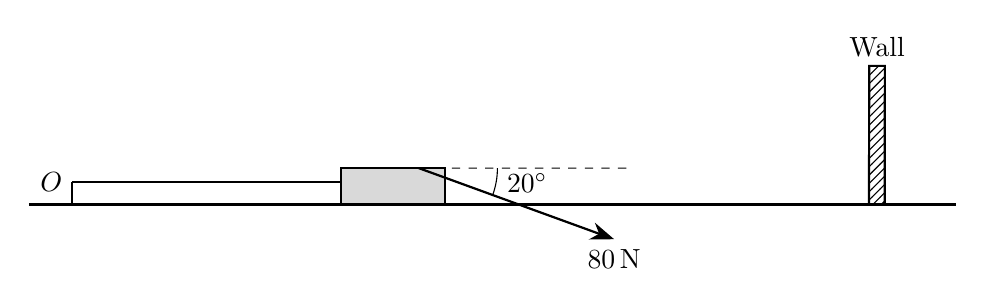
\begin{tikzpicture}[scale=1.1]
\def\surfL{-0.5}
\def\surfR{10.2}
\def\wallx{9.2}
\def\wallw{0.18}
\def\wallh{1.6}
\def\anchory{0.26}
\def\blockx{3.1}
\def\bw{1.2}
\def\bh{0.42}
\def\forceang{-20}
\def\forcelen{2.4}
\def\reflen{2.4}

\coordinate (S0) at (\surfL,0);
\coordinate (S1) at (\surfR,0);
\coordinate (A0) at (0,0);
\coordinate (O) at (0,\anchory);
\coordinate (BL) at (\blockx,0);
\coordinate (BR) at ($(BL)+(\bw,0)$);
\coordinate (TL) at ($(BL)+(0,\bh)$);
\coordinate (TR) at ($(BR)+(0,\bh)$);
\coordinate (Attach) at ($(BL)+(0,\anchory)$);
\coordinate (P) at ($(TL)!0.75!(TR)$);
\coordinate (H) at ($(P)+(\reflen,0)$);
\coordinate (F) at ($(P)+(\forceang:\forcelen)$);
\coordinate (WBL) at (\wallx,0);
\coordinate (WBR) at ($(WBL)+(\wallw,0)$);
\coordinate (WTL) at ($(WBL)+(0,\wallh)$);
\coordinate (WTR) at ($(WBR)+(0,\wallh)$);

\draw[thick] (S0) -- (S1);
\draw[thick] (A0) -- (O);
\draw[thick] (O) -- (Attach);
\draw[thick, fill=gray!30] (BL) rectangle (TR);

\fill[pattern=north east lines] (WBL) rectangle (WTR);
\draw[thick] (WBL) -- (WTL) -- (WTR) -- (WBR);

\draw[dashed] (P) -- (H);
\draw[-{Stealth[length=3mm]}, thick] (P) -- (F) node[below] {$80\,\mathrm{N}$};
\pic["$20^\circ$" {yshift=1.5pt}, draw, angle radius=10mm, angle eccentricity=1.4]
  {angle=F--P--H};

\node[left] at (O) {$O$};
\node[above] at ($(WTL)!0.5!(WTR)$) {Wall};
\end{tikzpicture}
\end{figure}


A block of mass $6\,\mathrm{kg}$ rests on a rough horizontal surface and is attached to a fixed point $O$ by a light elastic string. Initially the block is at rest $2.4\,\mathrm{m}$ from $O$. \\

The elastic string has natural length $2\,\mathrm{m}$ and modulus of elasticity $80\,\mathrm{N}$. \\

The coefficient of friction between the block and the surface is $0.25$. \\
A force of magnitude $80\,\mathrm{N}$ is applied to the block towards a vertical wall. The force acts at an angle of $20^\circ$ below the horizontal, as shown in the diagram. \\

The block moves in a straight line perpendicular to the wall, and the wall is sufficiently far away that the block does not reach it during the motion considered. \\
\begin{enumerate}[label=\textbf{(\alph*)}]
  \item Show that the block has moved $0.94\,\mathrm{m}$, correct to 2 significant figures, when the forces acting on it are in equilibrium. \marks{4} \\
  \item State one limitation of the model. \marks{1} \\
  \item Find the maximum speed of the block. \marks{4} \\
\end{enumerate}

\vspace*{10pt}

\begin{tcolorbox}[colback=white, colframe=scarlet, title={\textbf{Solution}}, breakable, grow to left by=6mm, grow to right by=10mm]
\begin{enumerate}[label=\textbf{(\alph*)}, start=1]
  \item Let the block move a distance \(x\,\mathrm{m}\) towards the wall.

  The string length is then \(2.4+x\), so its extension is
  \[
  (2.4+x)-2=0.4+x
  \]

  Hence the tension is
  \[
  T=\frac{\lambda}{l}e=\frac{80}{2}(0.4+x)=16+40x
  \]

  Since the block moves horizontally, it is in vertical equilibrium, so
  \[
  R=6g+80\sin 20^\circ=58.8+80\sin 20^\circ
  \]

  Therefore the friction is
  \[
  F=\mu R=0.25(58.8+80\sin 20^\circ)=21.54\,\mathrm{N}
  \]

  When the forces are in equilibrium, the horizontal forces balance:
  \begin{align*}
  80\cos 20^\circ &= T+F\\
  80\cos 20^\circ &= (16+40x)+21.54
  \end{align*}

  So
  \begin{align*}
  40x &= 80\cos 20^\circ-37.54\\
  x &\approx 0.9409
  \end{align*}

  Hence the block has moved \(0.94\,\mathrm{m}\), correct to 2 significant figures.

  \item One limitation is that the coefficient of friction is assumed to remain constant throughout the motion.

  \item From part (a), the equilibrium position is at \(x=0.9409\,\mathrm{m}\).

  At a general position \(x\), the horizontal resultant force is
  \[
  80\cos 20^\circ-21.54-(16+40x)=37.64-40x
  \]

  This decreases as \(x\) increases. It is positive initially, and it becomes zero when \(x=0.9409\). So the speed increases up to this point and then decreases afterwards. Hence the maximum speed occurs when \(x=0.9409\,\mathrm{m}\).

  Initially the extension is \(0.4\,\mathrm{m}\), so
  \[
  EPE_0=\frac{\lambda e^2}{2l}=\frac{80(0.4)^2}{2\times 2}=3.2\,\mathrm{J}
  \]

  At the position of maximum speed, the extension is
  \[
  e_1=0.4+0.9409=1.3409
  \]

  Using
  \[
  KE_0+GPE_0+EPE_0+\sum W_{\text{other}}=KE_1+GPE_1+EPE_1
  \]

  There is no change in GPE, the applied force does work \(80\cos 20^\circ\times 0.9409\), and friction does work \(-21.54\times 0.9409\).

  Therefore
  \begin{align*}
  0+3.2+80\cos 20^\circ(0.9409)-21.54(0.9409)
  &=\frac12(6)v^2+\frac{80(1.3409)^2}{2\times 2}\\
  53.66&=3v^2+35.96\\
  3v^2&=17.70\\
  v&=2.43\,\mathrm{m\,s^{-1}}
  \end{align*}

  So the maximum speed is \(2.43\,\mathrm{m\,s^{-1}}\).
\end{enumerate}
\end{tcolorbox}


\end{enumerate}
\end{document}
